\task{Без нулей}

\vspace{-0.2cm} \rightline{\itshape Двадцать восемь, двадцать девять, двадцать десять...}

\ms Рассмотрим обыкновенную десятичную систему счисления и то, как в ней записываются натуральные числа. Мы хотим найти способ избавиться от нулей в записи этих чисел. Давайте вместо нуля введём цифру «десять», которую будем записывать как {\verb!X!} и употреблять наравне с другими цифрами. После такой модификации системы счисления число 30, например, станет записываться как {\verb!2X!}, число 100 — как {\verb!9X!}, число 3107 — как {\verb!2XX7!}.

\begin{enumerate}

\item Переведите числа 110, 2202, 500'000 из десятичной системы счисления в модифицированную. Переведите числа {\verb!1X17!}, {\verb!XXXX!}, {\verb!512!} из модифицированной системы счисления в десятичную.

\item Объясните, почему всякое число имеет единственную запись в нашей модифицированной системе счисления.

\item Опишите алгоритм перевода чисел из десятичной системы в модифицированную и обратно.

\item Докажите, что запись числа в модифицированной системе счисления всегда не длиннее его записи в десятичной. Приведите пример, когда она строго короче десятичной.

\item Опишите правила сложения и умножения в столбик в модифицированной системе счисления (см.\,рис.\,R). Отличаются ли они от правил в обыкновенной десятичной системе?

\vspace{-0.3cm}
\begin{center}
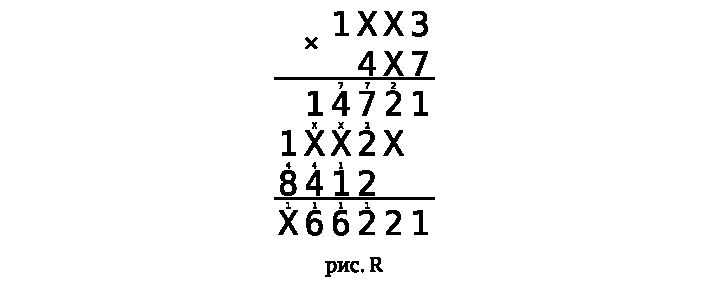
\includegraphics[width=10.5cm]{stats/2017/images/stolbik.pdf}
\end{center} \vspace{-0.7cm}

\item Придумайте способ распространить модифицированную систему счисления и на неположительные числа. В частности, как записать ноль в этой системе счисления?

\item В модифицированной системе счисления попробуйте сформулировать признаки делимости на
\subitem — 2, 4, произвольную степень двойки\scolon
\subitem — 5, 25, произвольную степень пятёрки\scolon
\subitem — 3, 9\scolon
\subitem — 11.

\item Что ещё можно сказать про модифицированную систему счисления? Как построить её аналог, используя двоичную систему вместо десятичной? Предложите свои направления исследования и изучите их.
\end{enumerate}